% !TeX document-id = {8751af90-d4b1-40f9-88be-89e61cd71d0c}
% !TeX TXS-program:compile = txs:///pdflatex/[--shell-escape]
\documentclass[a4paper,11pt]{article}

%\usepackage[style=apa]{biblatex}
\usepackage[style=apa,sortcites=true,sorting=nyt,backend=biber]{biblatex}
\usepackage{amsmath,amsfonts,amssymb, bm}
\usepackage{graphicx,verbatimbox}
\usepackage[colorlinks=true, allcolors=blue]{hyperref}
\usepackage{authblk}
\usepackage{nicefrac}
\usepackage{svg}

%opening
\title{Augmenting Predictive Models in Forensic Psychiatry with Cultural Consensus Theory}
\author[1]{Don van den Bergh}
\author[2]{Erwin Schuringa}
\author[1]{Eric-Jan Wagenmakers}
\affil[1]{Department of Psychological Methods, University of Amsterdam}
\affil[2]{Forensic Psychiatric Centre Dr. S. van Mesdag}
\date{}

%\usepackage[dvipsnames]{xcolor}
\usepackage{xcolor}
\usepackage{todonotes}

\definecolor{colorDon}{RGB}{205,250,255}
\definecolor{colorEJ} {RGB}{205,255,205}

\newcommand{\DB}[1]{\todo[inline, color=colorDon]{DB: {#1}}}
\newcommand{\EJ}[1]{\todo[inline, color=colorEJ]{EJ: {#1}}}

%\graphicspath{../figures}
\graphicspath{{../figures/}{../graphicalmodels/}}

\addbibresource{references.bib}


\newcommand{\Irater}{r}
\newcommand{\Iitem}{i}
\newcommand{\Ipatient}{p}
%\newcommand{\Incat}{c}
%\newcommand{\Ilatent}{l}
%\newcommand{\IdiscreteP}{d}
\newcommand{\Icovariate}{c}

\newcommand{\Trater}{\expandafter\MakeUppercase\expandafter{\Irater}}
\newcommand{\Titem}{\expandafter\MakeUppercase\expandafter{\Iitem}}
\newcommand{\Tpatient}{\expandafter\MakeUppercase\expandafter{\Ipatient}}
%\newcommand{\Tncat}{\expandafter\MakeUppercase\expandafter{\Incat}}
%\newcommand{\Tlatent}{\expandafter\MakeUppercase\expandafter{\Ilatent}}
%\newcommand{\TdiscreteP}{\expandafter\MakeUppercase\expandafter{\IdiscreteP}}
\newcommand{\Tcovariate}{\expandafter\MakeUppercase\expandafter{\Icovariate}}

% definitions of variables
\newcommand{\ItemTruth}{\theta}
\newcommand{\ItemDifficulty}{\kappa}
\newcommand{\UnBiasedThreshold}{\gamma}
\newcommand{\Threshold}{\delta}
\newcommand{\RaterScale}{\alpha}
\newcommand{\RaterShift}{\beta}
\newcommand{\RaterCompetence}{\zeta}
\newcommand{\Appraisal}{y}
\newcommand{\Error}{\epsilon}
\newcommand{\FactorScore}{\eta}
\newcommand{\FactorRegression}{\lambda}
%\newcommand{\RaterCovariate}{z}
%\newcommand{\PatientCovariate}{w}
\newcommand{\Covariate}{z}

\newcommand{\CovariateBeta}{\delta}
\newcommand{\ItemCovariateBeta}{\gamma}


% Probability distributions

%\newcommand{\ilogit}[1]{\text{logit}^{-1}\left(#1\right)}
\newcommand{\ilogit}[1]{\begin{revision}F\end{revision}\left(#1\right)}
\newcommand{\logit}[1]{\text{logit}\left(#1\right)}
\newcommand{\dnorm}[2]{\text{Normal}\left(#1,\,#2\right)}
\newcommand{\dnormp}[2]{\text{Normal\textsuperscript{+}}\left(#1,\,#2\right)}
\newcommand{\dgamma}[2]{\text{Gamma}\left(#1,\,#2\right)}
\newcommand{\dgammaMV}[2]{\text{Gamma}\left(\nicefrac{#1^2}{#2},\,\nicefrac{#1}{#2}\right)} % #1 is mean, #2 is variance
\newcommand{\dlognormal}[2]{\ensuremath{\mathrm{LogNormal}\left(#1,\,#2\right)}}
\newcommand{\dlogis}[2]{\text{Logistic}\left(#1,\,#2\right)}
\newcommand{\dlogiss}[3]{\text{Logistic}\left(#1;\,#2,\,#3\right)}

\newcommand{\dinvgamma}[2]{\text{InverseGamma}\left(#1,\,#2\right)}

% math commands
\newcommand{\assignment}{=}
\newcommand{\SE}[1]{\emph{({#1})}}
\newcommand{\code}[1]{\texttt{#1}}

% spaces
\newcommand{\Reals}{\mathbb{R}}
\newcommand{\PositiveReals}{\Reals^+}

% abbreviation Anders & Batchelder (2015)
\newcommand{\AB}{AB}


\begin{document}

\maketitle

\tableofcontents

\begin{abstract}

\end{abstract}

\section{Introduction}
The mental health and forensic risk factors of patients in forensic psychiatric hospitals is regularly monitored with methods such as
Routine Outcome Monitoring \parencite{deBeurs2011ROM}.
A staff member (e.g., a clinician or psychiatrist), henceforth a \emph{rater}, scores a patient on variety of criteria, such as ....
Using these scores raters can monitor the mental state of a patient over time, answer questions about the effectiveness of a treatment, or warn staff members about which patients are at risk for turning violent. 


For each patient, there are usually multiple scores available on different items, given by different raters.
The added value of the scores hinges on the method used to aggregate the scores.
Standard practice is to average the scores.
This is suboptimal, as this treats raters as exchangeable and analyzes patients independently.


In previous work, we used Cultural Consensus Theory \parencite[CCT;][]{romney1986culture, batchelder1988test, batchelder2012cultural} to develop an appropriate model to analyze such data that accounts for the hierarchical structure among patients, raters, and items \parencite{vandenBergh2020cultural}.
Here, we apply this model to data and uses its inferences to predict whether or not a patient becomes violent.
Furthermore, we compare the predictive performance to that of frequently used machine learning models.
In addition, we interpret the model and ...
The paper is concluded with a discussion on ...


\section{Data of 105 patients in the Mesdag clinic}
\subsection{Method of collection}
\subsection{IFTE}

The data were collected using a Routine Outcome Monitoring instrument called the the Instrument for Forensic Treatment Evaluation (IFTE).
The IFTE consists of 22 items, of which 14 items are criminogenic need indicators of the Dutch risk assessment instrument HKT-R \parencite{spreen2013handleiding}, five items were designed in consultation with psychologists and psychiatrists, and three items are based on the Atascadero Skills Profile \parencite{vess2001development}.
The 22 items can be grouped into three factors, Protective behaviors, Problematic behaviors, and Resocialization Skills.
All items are scored on a 17 point scale.

%\begin{quote}
%The Instrument for Forensic Treatment Evaluation is a multidisciplinary Routine Outcome Monitoring instrument. The IFTE is filled out in approximately 10 min every six months by all members of a patient's treatment team independently. The IFTE contains 22 indicators, comprising all 14 clinical criminogenic need indicators of the Dutch risk assessment instrument HKT-R (Spreen et al., 2014), three indicators based on the Atascadero Skills Profile (ASP; Vess, 2001), and five indicators designed in consultation with psychologists and psychiatrists. The 22 IFTE indicators are divided into three factors, namely Protective behaviors, Problematic behaviors and Resocialization Skills. Indicators of the IFTE are measured on a 17-point scale.
%\end{quote}


\subsection{Descriptive Statistics}
\begin{itemize}
	\item Amount of patients, raters, and items.
	\item Sparsity of patient-rater combinations.
\end{itemize}


\section{Cultural Consensus Theory}

Cultural Consensus Theory (CCT) sometimes called also known as ``test theory without an answer key'' \parencite{batchelder1988test}, is a method to discover the ''true answer`` for items from the consensus among the responses.
For example, suppose a mentally ill patient is scored by multiple raters on aggressiveness.
Multiple scores are obtained that need to be aggregated to arrive at a single score for this patient.
The naive solution is to average these scores.
However, as shown in Figure~\ref{fig:misFitMean} averaging may lead to severely biased estimates.
\DB{Figure here of score means versus true latent parameter for data simulated under the LTM.}
The average score disregards all additional information that is available.
It ignores the individual differences between raters, for example, this assumes that all psychiatrists score aggressiveness in the same way, and group differences among raters, for example, there is no difference in scores by psychiatrists as opposed to clinicians, or other staff member.
In addition, the average ignores any additional information about the patient at hand, such as the committed crimes and diagnoses.
\begin{figure}
	\centering
	\includesvg[width=\textwidth]{misfitMean}
	\caption{True item scores (x-axis) versus the sample mean across raters (y-axis).}
	\label{fig:misFitMean}
\end{figure}

Cultural consensus theory (CCT) provides a model-based framework for pooling information from multiple raters to form a consensus \parencite{anders2014cultural}.
There exist a variety of CCT models, each applicable to different types of data.
For example, the General Condorcet model \parencite{Batchelder1986statistical} applies to dichotomous data, the Latent Truth Rater model \parencite{Anders2015cultural} is suited for ordinal data, and the Continous Response model \parencite{anders2014cultural}.

\iffalse
\subsection{The Continuous Response Model}
The Continuous Response Model (CRM) is a CCT model for continuous data \parencite{anders2014cultural}.
Figure~\ref{model:CRM_p} shows a graphical model of the CRM with a few adjustments.

%\begin{figure}[!ht]
%	\begin{minipage}{0.5\textwidth}
%		\centering
%		\includegraphics[width=\textwidth, page=1]{../graphicalmodels/graphicalmodels.pdf}
%	\end{minipage}\hfill
%	\begin{minipage}{0.5\textwidth}
%		{\normalsize
%			\begin{align*}
%			x_{\Iitem\Irater}      			&\sim \dnorm{\mu_{\Iitem\Irater}}{\sigma^2_{\Iitem\Irater}} \\
%			\mu_{\Iitem\Irater}    			&\assignment \RaterScale_\Irater \ItemTruth_{\Iitem} + \RaterShift_\Irater  \\
%			\sigma_{\Iitem\Irater} 			&\assignment \RaterCompetence_\Irater \ItemDifficulty_\Iitem\\
%			\ItemTruth_\Iitem	   			&\sim \dnorm{\mu_\ItemTruth}{\sigma^2_\ItemTruth}\\
%			\log \ItemDifficulty_\Iitem 	&\sim \dnorm{\mu_\ItemDifficulty}{\sigma^2_\ItemDifficulty}\\
%			\log \RaterScale_\Irater     	&\sim \dnorm{\mu_\RaterScale}{\sigma^2_\RaterScale}\\
%			\RaterShift_\Irater	   			&\sim \dnorm{\mu_\RaterShift}{\sigma^2_\RaterShift}\\
%			\log \RaterCompetence_\Irater	&\sim \dnorm{\mu_\RaterCompetence}{\sigma^2_\RaterCompetence}\\
%			\end{align*}
%		}%
%	\end{minipage}
%	\caption{Graphical model of the Continuous Response Model for a single patient.}
%	\label{model:CRM_1}
%\end{figure}

\begin{figure}[!ht]
	\begin{minipage}{0.5\textwidth}
		\centering
		\includegraphics[width=\textwidth, page=3]{graphicalmodels.pdf}
	\end{minipage}\hfill
	\begin{minipage}{0.5\textwidth}
		{\normalsize
			\begin{align*}
			x_{\Ipatient\Iitem\Irater}      &\sim \dnorm{\mu_{\Ipatient\Iitem\Irater}}{\sigma^2_{\Ipatient\Iitem\Irater}} \\
			\mu_{\Ipatient\Iitem\Irater}    &\assignment \RaterScale_\Irater \ItemTruth_{\Ipatient\Iitem} + \RaterShift_\Irater  \\
			\sigma_{\Iitem\Irater} 			&\assignment \RaterCompetence_\Irater \ItemDifficulty_\Iitem\\
			\ItemTruth_{\Ipatient\Iitem}	&\sim \dnorm{\mu_\ItemTruth}{\sigma^2_\ItemTruth}\\
			\log \ItemDifficulty_\Iitem 	&\sim \dnorm{\mu_\ItemDifficulty}{\sigma^2_\ItemDifficulty}\\
			\log \RaterScale_\Irater     	&\sim \dnorm{\mu_\RaterScale}{\sigma^2_\RaterScale}\\
			\RaterShift_\Irater	   			&\sim \dnorm{\mu_\RaterShift}{\sigma^2_\RaterShift}\\
			\log \RaterCompetence_\Irater	&\sim \dnorm{\mu_\RaterCompetence}{\sigma^2_\RaterCompetence}\\
			\end{align*}
		}%
	\end{minipage}
	\caption{Graphical model of the Continuous Response Model for multiple patients.}
	\label{model:CRM_p}
\end{figure}
Here, $x_{\Ipatient\Iitem\Irater}$ is the score given to patient $\Ipatient$ on item $\Iitem$ by rater $\Irater$.
This score is assumed to be normally distributed with mean $\mu_{\Ipatient\Iitem\Irater}$ and standard deviation $\sigma_{\Iitem\Irater}$.
The mean is composed of a patients true score on a particular item $\ItemTruth_{\Ipatient\Iitem}$ and a rater-specific scale $\RaterScale_\Irater$ and shift $\RaterShift_\Irater$.
The standard deviation is comprised of an item-specific difficulty $\ItemDifficulty_\Iitem$ and a rater-specific competence $\RaterCompetence_\Irater$.
The ratio of the item difficulty and rater competence determines how precise an answer is retrieved.

There are three differences in Figure~\ref{model:CRM_p} compared to the CRM as described in \textcite{anders2014cultural}.
First, we do not allow for multiple cultural truths among the raters.
In our application the raters are professionally trained and we believe the remaining rater parameters suffice to capture differences between raters.
Second, \parencite{anders2014cultural} considered two levels of nesting, items and respondents, whereas we consider three levels of nesting, patients, items, and raters.
By dropping the patient indices one

Third, we adjusted the prior distributions opposed


Different cultural truths allows the ``true answer'' on an item to vary across patients
Another difference with respect to our previous work \parencite{vandenBergh2020cultural} is that the item difficulty $\ItemDifficulty$ does not vary across patients.
During simulations with a similar ratio of patients to raters, we found that this parameter cannot be reliably estimated.
Therefore we opted to constrain this parameter across patients.
\fi

\subsection{The Latent Truth Rater Model}
The Latent Truth Rater Model (LTM) is a CCT model for ordinal data \parencite{Anders2015cultural}.
Previously, we extended the LTM to handle data from multiple patients \parencite{vandenBergh2020cultural} and Figure~\ref{model:LTM_p} shows the LTM for multiple patients.
\begin{figure}[!ht]
	\begin{minipage}{0.55\textwidth}
		\centering
		\includegraphics[width=\textwidth, page=7]{graphicalmodels.pdf}
	\end{minipage}\hfill
	\begin{minipage}{0.45\textwidth}
		{\normalsize
			\begin{align*}
			\oneScore &\assignment
			\begin{cases}
			1		&\hspace{-.3cm} \text{if } \oneAppraisal \leq \Threshold_{\Irater 1} \\
			\Incat	&\hspace{-.3cm} \text{if } \Threshold_{\Irater, \Incat-1} < \oneAppraisal \leq \Threshold_{\Irater\Incat} \\
			\Tncat	&\hspace{-.3cm} \text{if } \oneAppraisal > \Threshold_{\Irater, \Tncat-1}
			\end{cases}\\
			\oneAppraisal &\sim \dlogis{\ItemTruth_{\Ipatient\Iitem}}{\nicefrac{\ItemDifficulty_\Iitem}{\RaterCompetence_\Irater}} \\
			\Threshold_{\Irater\Incat} &\sim \dnorm{0}{1}\\
			\ItemTruth_{\Ipatient\Iitem}        &\sim \dnorm{\mu_\ItemTruth}{\sigma_\ItemTruth^2}\\
			\ItemDifficulty_\Iitem   &\sim \dgammaMV{\mu_\ItemDifficulty}{\sigma_\ItemDifficulty^2} \\
			\RaterCompetence_\Irater &\sim \dgammaMV{\mu_{\RaterCompetence_\Irater}}{\sigma_{\RaterCompetence_\Irater}^2} \\
			\end{align*}
		}%
	\end{minipage}
	\caption{%
		Graphical model of the Latent Truth Rater Model for multiple patients.
		Note that the thresholds $\bm{\Threshold}_\Irater$ are constrained to be ordered, that is, for all raters we have $\Threshold_{\Irater 1} \leq \dots \leq \Threshold_{\Irater \Incat} \leq \dots \leq \Threshold_{\Irater,\Tncat-1}$.
	}
	\label{model:LTM_p}
\end{figure}

Here, $\oneScore$ is the observed score given to patient $\Ipatient$ on item $\Iitem$ by rater $\Irater$.
This score is assumed to be deterministically generated from a continuous latent appraisal $\Appraisal_{\Ipatient\Iitem\Irater}$ that is discretized to an ordinal scale by the thresholds $\Threshold_{\Irater\Incat}$.
In particular, we have that
\begin{align*}
\oneScore =
\left\{\begin{array}{ll}
1		& \text{if }  \Appraisal_{\Ipatient\Iitem\Irater} \leq \Threshold_{\Irater 1} \\[4pt]
\Incat	& \text{if }  \Threshold_{\Irater, \Incat - 1} < \Appraisal_{\Ipatient\Iitem\Irater} \leq \Threshold_{\Irater\Incat} \\[4pt]
\Tncat	& \text{if }  \Appraisal_{\Ipatient\Iitem\Irater} > \Threshold_{\Irater,\Tncat-1}
\end{array} \right.
\end{align*}
Since the appraisal score is latent, the deterministic function above implies the following probabilistic model over the observed scores:
\begin{align*}
P(\oneScore\mid \oneAppraisal,\bm{\Threshold}_{\Irater}) =
\left\{\begin{array}{ll}
1 - \cdf{\Appraisal_{\Ipatient\Iitem\Irater} - \Threshold_{\Irater 1}}         & \text{if } \oneScore = 1, \\[4pt]
\cdf{\oneAppraisal - \Threshold_{\Irater,\Incat-1}} -
\cdf{\oneAppraisal - \Threshold_{\Irater\Incat}}         & \text{if } 1 < \oneScore < \Tncat,\\[4pt]
\cdf{\oneAppraisal - \Threshold_{\Irater,\Tncat-1}}       & \text{if } \oneScore = \Tncat.
\end{array} \right.
\end{align*}
where $\cdf{}$ is the logistic cumulative distribution function.\footnote{%
	Note that this choice is arbitrary and that it is possibly to use any continuous cumulative distribution function.
}

Next, we explain how the latent appraisals and thresholds come about.
The appraisals are draws from a logistic distribution with location $\ItemTruth_{\Ipatient\Iitem}$, the true score for patient $\Ipatient$ on item $\Iitem$. The scale of the logistic distribution is the ratio of the item difficulty $\ItemDifficulty_\Iitem$ to the rater competence $\RaterCompetence_\Irater$.
A higher item difficulty means that the appraisals are more noisy, which leads to a more dispersed probability distribution over possible scores.
Conversely, a higher rater competence means that the appraisals are less noisy, which leads to a more concentrated distribution over the outcomes.
There are $\Tncat - 1$ ordered thresholds for each rater, which are assigned a standard normal prior for identification purposes.

There are two differences in the model specification above compared to our previous work \parencite{vandenBergh2020cultural}.
%We made two changes to the model, because when simulating data with similar characteristics as the Mesdag data, as
First, we previously modeled the thresholds using two rater specific parameters.
However, in simulations we noticed that these two parameters provide too little flexibility when the ordinal scale consists of 18 categories, as in the Mesdag data.
Therefore we decided to model the thresholds individually.
This complicates interpreting the differences between the thresholds across raters, however, that is also not the goal of this paper.
Second, we previously allowed the item difficulty parameter to vary across patients, which captures that some items may be more difficulty or easy to assess for some patients (e.g., some patients may cooperate more than others).
This parameter is mainly informed by the number or raters and there needs to be a sufficient amount of raters that score each patient for a reliable estimate.
However, we noticed when simulating data with a ratio of raters to patients like in the data at hand that there are simply too few observations to reliably estimate the deviations in item difficulty across patients.
% \DB{We could also look at a patient specific ``cooperativeness'' parameter. Rather than doing $\ItemDifficulty_{\Ipatient\Iitem}$, which introduces $\Tpatient\times\Titem$ parameters, the logistic scale would become $\frac{\ItemDifficulty_\Iitem}{\RaterCompetence_\Irater \times\text{Cooperativeness}_\Ipatient}$. This introduces an additional $\Tpatient$ parameters.}


%$\Appraisal_{\Ipatient\Iitem\Irater} \leq \Threshold_{\Irater1}$ implies that $x_{\Ipatient\Iitem\Irater} = 1$, $\Threshold_{\Irater, \Incat - 1} < \Appraisal_{\Ipatient\Iitem\Irater} \leq \Threshold_{\Irater\Incat}$ implies that $x_{\Ipatient\Iitem\Irater} = \Incat$, and $\Appraisal_{\Ipatient\Iitem\Irater} > \Threshold_{\Irater\Tncat}$ implies that $x_{\Ipatient\Iitem\Irater} = \Tncat$.
%
%  that distributed with mean $\mu_{\Ipatient\Iitem\Irater}$ and standard deviation $\sigma_{\Iitem\Irater}$.
%
%
%Compared to our previous work, we made a few adjustments to make the model more suited for analyzing the data at hand.
%First, we removed
%
%
%Previously we modeled the thresholds using two rater specific parameters. However, during simulations we noticed that this is too restrictive when the ordinal scale consists of 18 categories, as in the data example at hand.


\subsection{Augmenting Logistic Regression with the LTM}
In a next step, we use logistic regression for to predict violent behavior, where we use the results from the LTM as additional predictors.
We do so in a fully Bayesian approach, that is, we constructed a joint model for the violent behavior and then patient ratings.%
\footnote{%
An alternative is to fit the LTM separately and then use e.g., the posterior means in a second step in a logistic regression.
While this would be more computationally efficient, it would also ignore the uncertainty in the analysis of the patient ratings.
}
Figure~\ref{model:Logistic_LTM} shows a graphical model of the logistic regression combined with the LTM.
The latent truth for each patient on each item is seen as a covariate in the logistic regression model.

%with a logistic regression
%In our application we are not directly interested in the results of the LTM, but rather, we wish to predict violent behavior
%The CRM applies an information pooling strategy. Here, we use the results from the CRM, specifically the item truths for each patient, to augment prediction of aggressiveness.

\begin{figure}[!ht]
%	\begin{minipage}{0.5\textwidth}
		\centering
		\includegraphics[width=\textwidth, page=8]{graphicalmodels.pdf}
%	\end{minipage}\hfill
%	\begin{minipage}{0.5\textwidth}
%		{\normalsize
%			\begin{align*}
%			x_{\Ipatient\Iitem\Irater}      &\sim \dnorm{\mu_{\Ipatient\Iitem\Irater}}{\sigma^2_{\Ipatient\Iitem\Irater}} \\
%			\mu_{\Ipatient\Iitem\Irater}    &\assignment \RaterScale_\Irater \ItemTruth_{\Ipatient\Iitem} + \RaterShift_\Irater  \\
%			\sigma_{\Iitem\Irater} 			&\assignment \RaterCompetence_\Irater \ItemDifficulty_\Iitem\\
%			\ItemTruth_{\Ipatient\Iitem}	&\sim \dnorm{\mu_\ItemTruth}{\sigma^2_\ItemTruth}\\
%			\log \ItemDifficulty_\Iitem 	&\sim \dnorm{\mu_\ItemDifficulty}{\sigma^2_\ItemDifficulty}\\
%			\log \RaterScale_\Irater     	&\sim \dnorm{\mu_\RaterScale}{\sigma^2_\RaterScale}\\
%			\RaterShift_\Irater	   			&\sim \dnorm{\mu_\RaterShift}{\sigma^2_\RaterShift}\\
%			\log \RaterCompetence_\Irater	&\sim \dnorm{\mu_\RaterCompetence}{\sigma^2_\RaterCompetence}\\
%			\end{align*}
%		}%
%	\end{minipage}
	\caption{Graphical model of Logistic Regression Augmented with the Latent Truth Rater Model.}
	\label{model:Logistic_LTM}
\end{figure}

\subsection{The Latent Truth Rater Model}

%\begin{figure}
%	\centering
%	\includegraphics[width=\textwidth, page=5]{graphicalmodels.pdf}
%	\caption{Graphical model of Logistic Regression Augmented with the Latent Truth Rater Model.}
%	\label{model:Logistic_LTM}
%\end{figure}
%
%\begin{figure}
%	\centering
%	\includegraphics[width=\textwidth, page=6]{graphicalmodels.pdf}
%	\caption{Graphical model of Logistic Regression Augmented with the Latent Truth Rater Model.}
%	\label{model:Logistic_LTM}
%\end{figure}

\subsection{Simulation Study}

Before analyzing the data with the LTM, it is typically a good idea to run a simulation study to

\subsubsection{Do we actually want to report this?}

\subsubsection{Fit of the LTM}



\subsection{Machine Learning Alternatives}
A
This section discusses the four alternative considered, naive logistic regression, random forest, boosted regression trees.


\subsubsection{Missing value imputation and data reduction}
The four machine learning methods described above are designed for purely rectangular data.
That is, each row of the data set contains one outcome (aggressive or not) and a number of predictors.
However, the raw data contains repeated observations.
For example, some patients were rated multiple times but others only once.
This means that some preprocessing of the data is needed before these methods can be applied.
Here we discuss missing data handling and the data reduction techniques applied.

\paragraph{Missing values}
The four alternative methods do not handle missing values.
Although list-wise deletion is an option, this may results in deleting many observations.
We used the R package \code{mice} \parencite{vanBuuren2011mice} to impute missing values.
%Rather than imputing one single value for each missing observation, \code{mice} imputes multiple, which leads to multiple data sets.
%While this increases the computational complexity of the procedures, it also propagates uncertainty about the missing observations to the results.


\paragraph{Data reduction}
After imputing missing values in the data, it remains problematic that there are multiple raters


\section{Empirical Example}

\subsection{Data set about Forensic Psychiatric}
doei
\subsection{Discussion}
Summary

Hybrid is probably most predictive.

\subsection{Suggestions for future data collection}



\subsection{Limitations}

\printbibliography

%\appendix
%\section{EM Algorithm}
%
%Initial values are found using a few steps of an EM-algorithm that disregards the priors and hyperparameters.
%\begin{align*}
%	\RaterShift_\Irater &\sim \prod_{\Ipatient=1}^\Tpatient\prod_{\Iitem=1}^\Titem \dnorm{x_{pir} - \RaterScale_\Irater\ItemTruth_{\Ipatient\Iitem}}{\left(\ItemDifficulty_\Iitem\RaterCompetence_\Irater\right)^2} \\
%	\RaterScale_\Irater &\sim \prod_{\Ipatient=1}^\Tpatient\prod_{\Iitem=1}^\Titem
%	\dnorm{\frac{
%			\RaterShift_\Irater - x_{pir}
%		}{
%			\ItemTruth_{\Ipatient\Iitem}
%		}}{
%		\left(\frac{
%			\ItemDifficulty_\Iitem\RaterCompetence_\Irater
%		}{
%			\left|\ItemTruth_{\Ipatient\Iitem}\right|}\right)^2
%		} \\
%	\ItemTruth_{\Ipatient\Iitem} &\sim \prod_{\Irater=1}^\Trater
%	\dnorm{\frac{
%			x_{pir} - \RaterShift_\Irater
%		}{
%			\RaterScale_\Irater
%		}}{
%		\left(\frac{
%			\ItemDifficulty_\Iitem\RaterCompetence_\Irater
%		}{
%			\RaterScale_\Irater}\right)^2
%	} \\
%	\RaterCompetence_\Irater^2 &\sim \dinvgamma{\frac{\Tpatient\Titem}{2}-1}{
%		\sum_{\Iitem=1}^\Titem \frac{1}{2\ItemDifficulty_\Iitem^{2}}\sum_{\Ipatient=1}^\Tpatient
%		\left(x_{pir} - \RaterScale_\Irater\ItemTruth_{\Ipatient\Iitem} - \RaterShift_\Irater\right)^2
%	}\\
%	\ItemDifficulty_\Iitem^2 &\sim \dinvgamma{\frac{\Tpatient\Trater}{2}-1}{
%		\sum_{\Irater=1}^\Trater \frac{1}{2\RaterCompetence_\Irater^{2}}\sum_{\Ipatient=1}^\Tpatient
%		\left(x_{pir} - \RaterScale_\Irater\ItemTruth_{\Ipatient\Iitem} - \RaterShift_\Irater\right)^2
%	}
%\end{align*}

\end{document}
